%نام و نام خانوادگی:
%شماره دانشجویی: 
\مسئله{ }

\پاسخ{}
\\

الف)
در ابتدا که مانند تمام حالات دیگر، fp
و ra
را تعین می‌کنیم.
\\
پس از آن با تابع
main
سر و کار داریم که خط به خط اجرا خواهد شد. بخش نخست
frame
stack 
نیز مختص این تابع است.
ابتدا مقادیر دو متغیر محلی 
a
و
b
 در سر استک قرار خواهند گرفت. در این حالت تابع main
 همان تابع caller
 ماست که این مقادیر را push
 می‌کند.
 سپس اجرای برنامه به تابع gcd
 می‌رسد.
 این مقدار نیز توسط تابع main
 مانند مقادیر قبلی در stack
 قرار می‌گیرد.
 \\
 سپس با فراخوانی تابع جدید، از تابع main خارج شده
 و برای نخستین بار با اجرای تابع gcd
 مقادیر را در استک قرار می‌دهیم.
 این بخش ، بخش دوم شکل ماست.
 در این حالت تابع main
 مقادیر x
 و
 y
 و 
 fp
 و
 ra
 را درون استک قرار خواهد داد.
مقادیری که این تابع در نهایت بازخواهد گرداند، توسط خود این تابع 
gcd
درون استک قرار داده خواهد شد. 
یعنی خطوط 8 و 11 توسط تابع gcd
که برای بار نخست صدا زده شده است ، پر می‌شوند.
\\
سپس مشابه بخش دوم، بخش سوم استک را هم پر می‌کنیم.
این بخش مربوط به اجرای تابع 
gcd
برای بار دوم است.
زمانی که برای اولین بار خط 11 ام برنامه اجرا شود،
خانه‌های 6ام به بعد استک نیز شروع به پر شدن می‌کنند.
سپس به جایی میرسیم که شرط اول تابع 
gcd
برقرار است و مجددا مقادیر قابل بازگشت در استک توسط خود تابع
gcd
در استک قرار می‌گیرند. یعنی خانه‌های 14 و 17.
لازم به ذکر است که این مقادیر توسط تابع gcd
نخست push می‌شوند.
\\
سپس تابع برای بار سوم اجرا شده و این را در بخش چهارم استک میبینید.
در این بخش هم 
مشابه بخش قبل مقادیر داخل استک قرار خواهند گرفت با این فرق که این بار تابع
gcd
دوم
این مقادیر را push
می‌کند.
لازم به ذکر است که اگر هر خانه را 4تایی فرض کنیم،
خانه اول اگر آدرسش x
باشد،
خانه‌های 9 ام و 15ام و 21 ام به ترتیب برابر 
x
و
x-28
و
x-48
خواهند شد.
\\
پس همانطور که پیش‌تر گفته شد،
که برای اولین بار خط 11 ام برنامه اجرا شود،
خانه‌های 6ام به بعد استک نیز شروع به پر شدن می‌کنند
\\
ب)
\\
توضیحات مانند قبل است.
با اتمام اجرای خط هشتم،
چون دیگر تابعی صدا زده نمیشود و مرحله به مرحله از هر تابع برمیگردیم تا تا کل استک از بالا به پایین 
رفته و به خط 5 میرسد و متغیر محلی
c
مقدار 12 را به خود می‌گیرد.

\begin{figure}[htp]
    \centering
    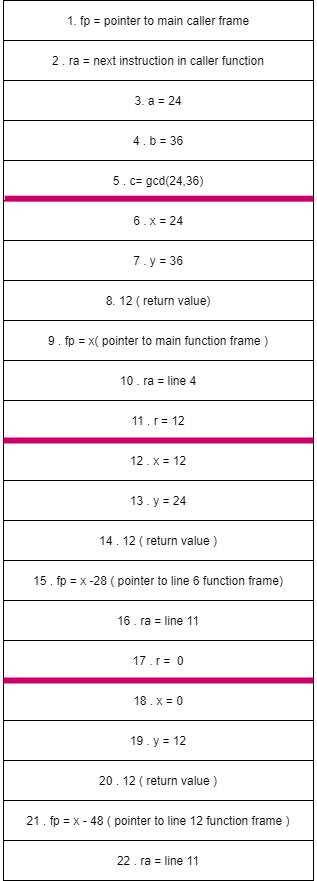
\includegraphics[width=8cm]{images/q2.png}
    \caption{frame Stack }
\end{figure}  